\chapter{Desenvolvimento}

\lipsum[1]

\section{Metodologia}

\lipsum[1]

\section{Simula{\c c}{\~a}o}

O objetivo proposto implica no treinamento de carros autônomos
que pudessem vir a ser dispostos em ambientes práticos de modo
a saber lidar com seus arredores e alcançar resultados
práticos. Seja o ambiente real uma réplica do circuito
presente na aplicação ou um ambiente novo, a validação dos
testes vem a acontecer em sua totalidade através de um
\textit{software} desenvolvido.

Este espaço virtual visa simular um carro dentro de um
circuito fechado cercado por paredes, o qual, pondo em prática
sua autonomia, está equipado de sensores que medem sua
distância ao bloqueio mais próximo à sua frente, e num
intervalo de 45° para ambos os lados até se tornarem
perpendiculares, somando-se assim cinco distâncias a serem
medidas. Na \autoref{fig_simul} pode-se observar a representa{\c c}{\~a}o gr{\'a}fica desse espa{\c c}o.

\begin{figure}[htb]
        \centering
        \caption{\label{fig_simul}Interface gráfica utilizada para a simulação, com o modelo de carro autônomo, trajeto de treino a ser percorrido e botões de controle de \textit{layout}.}
        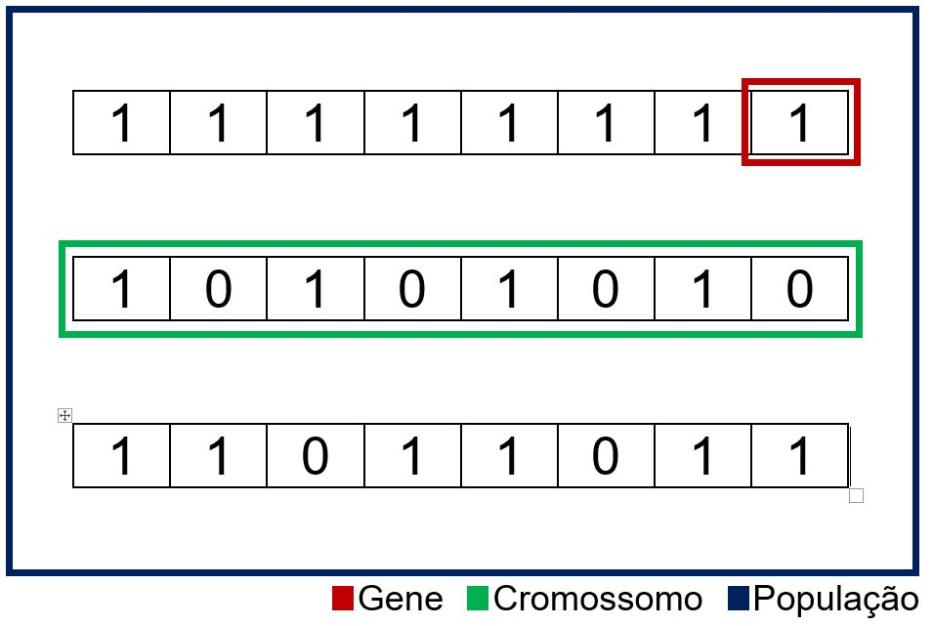
\includegraphics[width=0.7\textwidth]{images/gene.jpg}
        \legend{
                Fonte: Autoria Pr{\'o}pria.
        }
\end{figure}

O ambiente de simulação utilizado como base para os
experimentos foi desenvolvido em python com a biblioteca
\textit{pygame}, sua interface oferece métodos baseando-se em
orientação a objeto para a elaboração de jogos e aplicações
multimídia, através desta se fez o design da janela de
execução com seus elementos de tela (botões e limites do
circuito). Em conjunto, se faz uso da biblioteca de física 2d
\textit{pymunk}, para controlar a movimentação e colisão do carro.

A configuração do carro, no que diz respeito à sua interação
com ambiente, engloba:

\begin{enumerate}
	\item A posição inicial do carro e a distância por ele percorrida, utilizadas posteriormente como indicadores de desempenho para o algoritmo de neuroevolução;
	\item A forma do carro, a princípio definida como um círculo para facilitar sua movimentação pelo espaço, evitando colisões involuntárias;
	\item Sensoriamento do carro, identificando sua distância às paredes, posteriormente sendo utilizado para tomadas de decisão.
\end{enumerate}
